\documentclass{beamer}
%\usepackage[utf8]{inputenc}
\usetheme{Frankfurt}
\usepackage{natbib}
\usepackage{graphicx}

\title{CRYPTOCURRENCY}
\author{Dhwani Agarwal}
\institute{Dept. of CE \& IT, VJTI, Mumbai \\ 
            ID No: 171081018 \\
            Professor: Pranav Nerurkar}
\begin{document}

\begin{frame}
  \titlepage
\end{frame}

\begin{frame}{Table Of Contents}
  \tableofcontents
\end{frame}

\section{Introduction}

\begin{frame}{Introduction}
   
      \textbf {Cryptocurrency} is a medium of exchange value that exists in the digital world, that relies on encryption, for secure transactions.
   
    \begin{figure}
    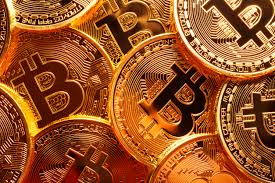
\includegraphics[width=1\textwidth, height=4.9cm,keepaspectratio]{images_bit.jpg}
    \caption{BitCoin}
    \source{Source : https://www.lifewire.com/what-are-bitcoins}
\end{figure}
\end{frame}

\section{Definition}

\begin{frame}{Definition}
    Below is a list of six things that every cryptocurrency must be in order for it to be called a cryptocurrency;
    \begin{itemize}
        \item \textbf{Digital:} Cryptocurrency only exists on computers. There are no coins and no notes. 
        \item \textbf{Decentralized:} Cryptocurrencies don’t have a central computer or server.
        \item \textbf{Peer-to-Peer:} Cryptocurrencies are passed from person to person online.There are no trusted third parties such as banks involved. 
        
    \end{itemize}
    
\end{frame}
\begin{frame}{}
    \begin{itemize}
        \item \textbf{Pseudonymous:} This means that you don’t have to give any personal information to own and use cryptocurrency. 
        \item \textbf{Trustless:} No trusted third parties means that users don’t have to trust the system for it to work. 
        \item \textbf{Encrypted:} Each user has special codes which stop their information from being accessed by other users. 
        \item \textbf{Global:} Cryptocurrencies can be sent all over the world easily.
    \end{itemize}
\end{frame}

\section{Story of Bitcoin}

\begin{frame}{Story of Bitcoin}
    \begin{itemize}
        \item In late 2008, \textit{\textbf{ Satoshi Nakamoto}} published the Bitcoin whitepaper.
        \item This was a description of what Bitcoin is and how it works.
        \item No one knows who Satoshi Nakamoto is. It could be a man, a woman or even a group of people. 
        \item On January 12, 2009, Satoshi Nakamoto made the first Bitcoin transaction. 
        \item They sent 10 BTC to a coder named Hal Finney.
        \item By 2011, Satoshi Nakamoto was gone. What they left behind was the world’s first cryptocurrency.
    \end{itemize}
\end{frame}

\section{What is BlockChain}

\begin{frame}{What is BlockChain}
    \begin{itemize}
        \item The thing that makes cryptocurrency different is blockchain technology.
        \item All cryptocurrencies use \textit{\textbf{ distributed ledger technology (DLT)}} to remove third parties from their systems. 
        \item DLTs are shared databases where transaction information is recorded.
        \item The DLT that most cryptocurrencies use is called blockchain technology.
        \item A blockchain is a database of every transaction that has ever happened using a particular cryptocurrency.
    \end{itemize}
\end{frame}

\begin{frame}{}
    \begin{itemize}
        \item So, a blockchain is a linear chain of blocks! 
        \item Once information is added to the blockchain, it can’t be deleted or changed.
        \item It stays on the blockchain forever and everyone can see it.
        \item New information can only be added to the blockchain if more than half of the nodes agree that it is valid and correct.
        \item This is called consensus.
        \item The idea of consensus is one of the big differences between cryptocurrency and normal banking.
    \end{itemize}
\end{frame}

\begin{frame}{}
     \begin{figure}
    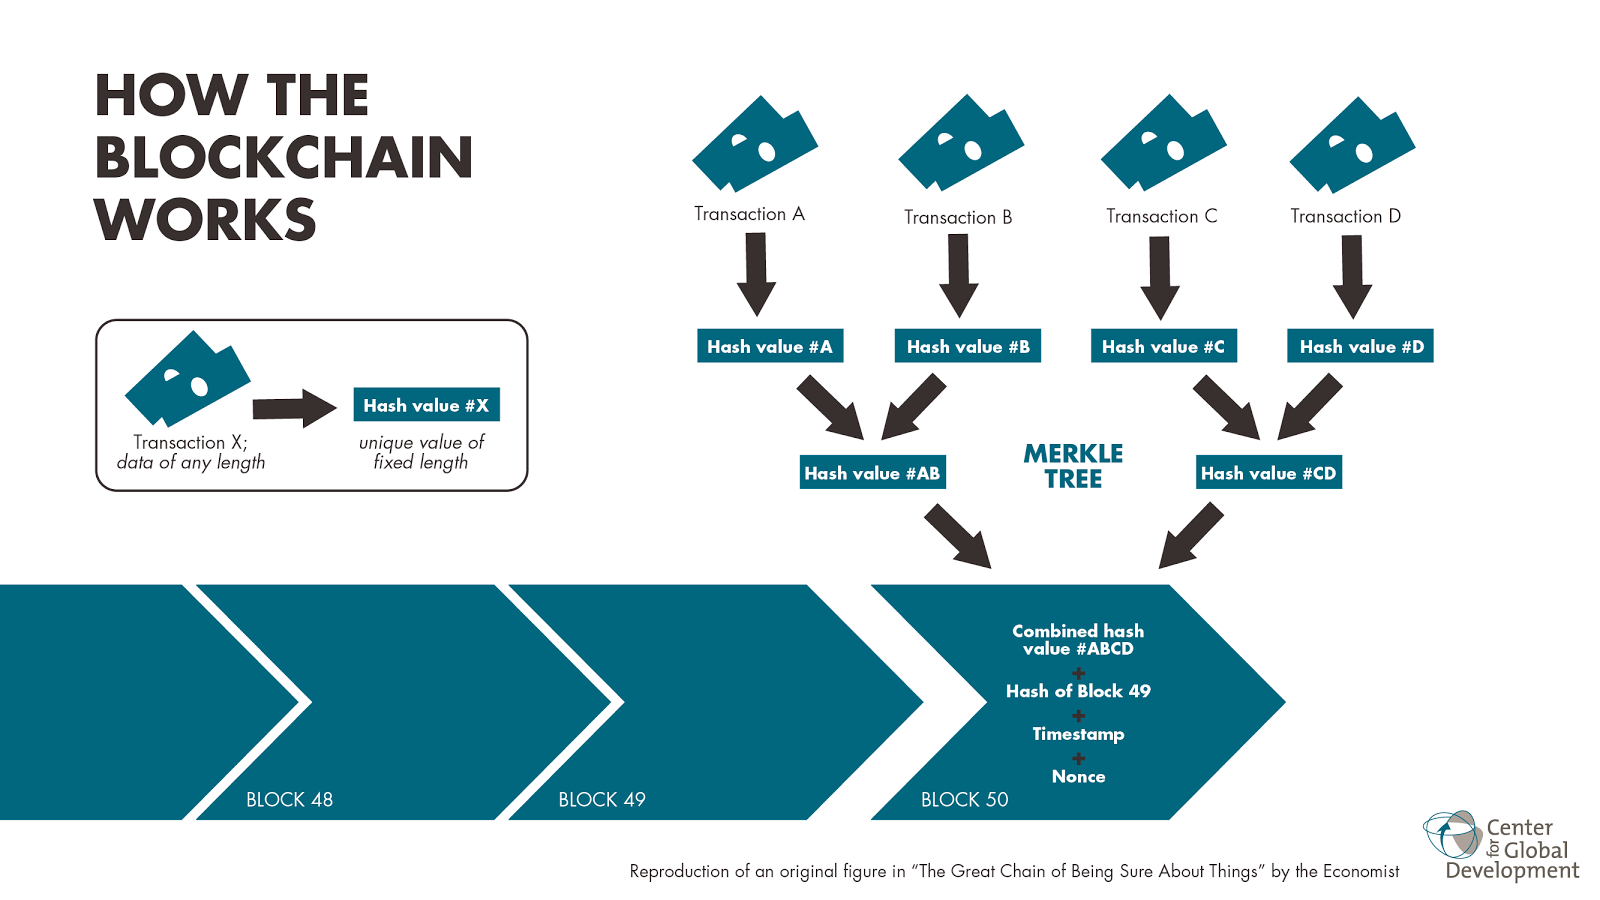
\includegraphics[width=1\textwidth]{blockchain.png}
    \caption{How BlockChain Works}
    \source{Source: https://blockgeeks.com/guides/what-is-blockchain-technology/}
\end{figure}
\end{frame}


\section{Cryptocurrency Mining}

\begin{frame}{Cryptocurrency Mining}
    \begin{itemize}
        \item Cryptocurrency transactions are verified by a process called mining.
        \item Cryptocurrency mining is actually more like accounting.
        \item Mining cryptocurrency uses a lot of computer power, so miners are rewarded for the work they do.
        \item On the Bitcoin network, miners who confirm new blocks of information are rewarded with 12.5 BTC of new Bitcoin.
        \item Current price of 1 BTC is \textbf{2,78,893} Indian rupees.
    \end{itemize}
      
\end{frame}


\begin{frame}{}
    \begin{figure}
    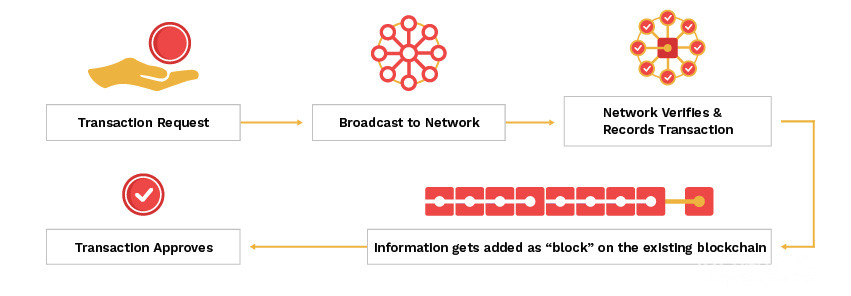
\includegraphics[width=1\textwidth]{what-is-cryptocurrency-7.jpg}
    \caption{Mining Process}
    \source{Source: https://www.bitdegree.org/tutorials/what-is-cryptocurrency/}
\end{figure}
\end{frame}

\section{Conclusion}

\begin{frame}{Conclusion}
\begin{itemize}
    \item Cryptocurrency is a radically new way of paying that makes all the transactions secure 
    \item It helps to get rid of intermediaries which contributes to a significant reduction in the commission fee. 
    \item The main feature of cryptocurrencies is security which is provided by Blockchain technology %— a network of computers having an identical copy of the database and changing its records by a common agreement based on pure mathematics. 
    \item Some other cryptocurrencies include : LiteCoin, Ethereum, IOTA etc.
\end{itemize} 
\end{frame}

\section{References}

\begin{frame}{References}
    \begin{thebibliography}{9}
    \bibitem{} https://www.bitdegree.org/tutorials/what-is-cryptocurrency
    \bibitem{} https://medium.com
    \bibitem{} Wikipedia
    \end{thebibliography}
\end{frame}

\end{document}
